\documentclass[12pt,twoside, a4paper, twocolumn]{article}
\usepackage[utf8]{inputenc}
\usepackage[brazil]{babel}
\usepackage[margin = 0.5in]{geometry}
\usepackage{amsmath}
\usepackage{amsthm}
\usepackage{amssymb}
\usepackage{amsthm}
\usepackage{setspace}
\usepackage[americanvoltages,fulldiodes,siunitx]{circuitikz}
\usepackage{lipsum}
\usepackage{pgfplots}
\usepackage{ifthen}
\usepackage{adjustbox}
\usepackage[section]{placeins}
\usepackage{hyperref}
\usepackage{graphicx}
\usepackage{amsmath}
\usepackage{amsthm}
\usepackage{amssymb}
\usepackage{amsthm}
\usepackage{setspace}
\usepackage[americanvoltages,fulldiodes,siunitx]{circuitikz}
\usepackage{lipsum}
\usepackage{pgfplots}
\usepackage{ifthen}
\usepackage{adjustbox}
\usepackage[section]{placeins}
\usepackage{hyperref}
\usepackage{graphicx}
\usepackage{adjustbox}
\pgfplotsset{compat=newest}
\graphicspath{ {./images/} }
%  #1 color - optional #2 x_0 #3 y_0 #4 x_f #5 y_f #6 name - optional  #7 true if adding lines to axis
\newcommand{\drawvector} [9] [color=cyan] {
  \draw[line width=1.5pt,#1,-stealth](axis cs: #2, #3)--(axis cs: #4, #5) node[anchor=south west]{$#6$};
 \ifthenelse{\equal{#7}{true}}{
  \draw[line width=1pt,#1, dashed](axis cs: #4, #5)--(axis cs: #4, 0) node[anchor= north west]{$#8$};
  \draw[line width=1pt,#1, dashed](axis cs: #4, #5)--(axis cs: 0, #5) node[anchor=south east]{$#9$};
  }
  {}
}
\newcommand\deriv[2]{\frac{\mathrm d #1}{\mathrm d #2}}
\title{Terceiro Relatório de Lab de Circuitos II}
\author{Henrique da Silva \\ hpsilva@proton.me}
\date{\today}
\pgfplotsset{width = 10cm, compat = 1.9}
\begin{document}
\maketitle
\pagenumbering{gobble}
\newpage
%pagenumbering{roman}
\tableofcontents
\newpage

\section{Introdução}


\subparagraph*{Neste relatório, vamos discutir calcular graficos de Bode de dois circuitos de segunda ordem e medir suas caracteristicas.}


\subparagraph*{Todos arquivos utilizados para criar este relatório, e o relatorio em si estão em:  \url{https://github.com/Shapis/ufpe_ee/tree/main/5th semester/Circuits II/}}








\section{Análise preliminar}


\paragraph*{Utilizarei o WxMaxima e LTSpice para fazer a análise teórica do circuito antes de montá-lo fisicamente.}


\paragraph*{Após terminar as análises compararei os resultados obtidos nas analises numericas e em laboratorio para verificar sua coerencia.}


\subsection{O Circuito}
\begin{adjustbox}{scale=0.30}
    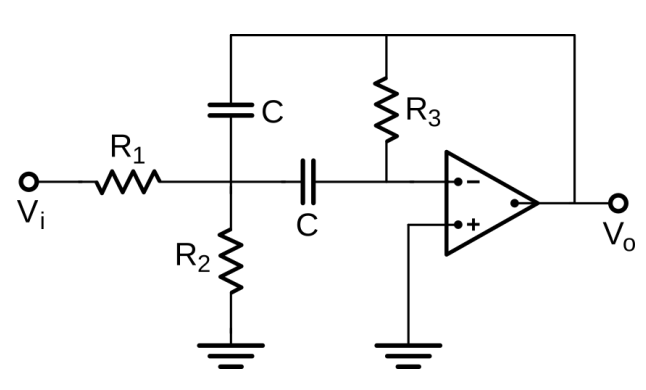
\includegraphics{AnaliseNodal.png}
\end{adjustbox}
\newpage
\subsection{WxMaxima}

\subsubsection{Analise geral do circuito}


\subparagraph*{Primeiro fiz manualmente a análise nodal do circuito que vamos construir, e passei ele para o domínio da frequência.}
\subparagraph*{}


\begin{adjustbox}{scale=0.4}
    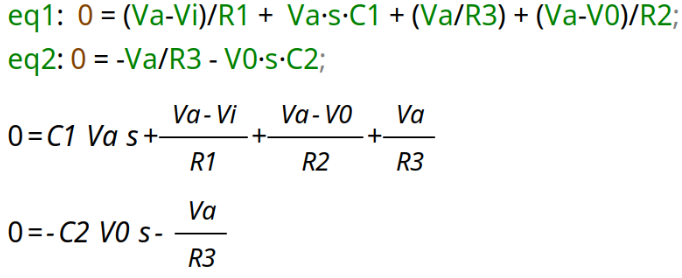
\includegraphics{eqs.png}
\end{adjustbox}


\subparagraph*{Após isso resolvi para $Va$ e $V_0$}


\subparagraph*{}


\begin{adjustbox}{scale=0.4}
    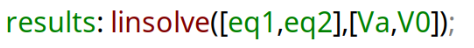
\includegraphics{linsolve.png}
\end{adjustbox}

\subparagraph*{}

\begin{adjustbox}{scale=0.4}
    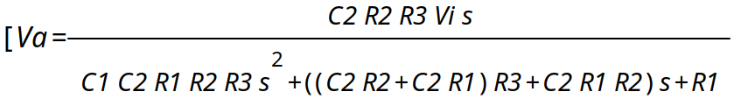
\includegraphics{va.png}
\end{adjustbox}

\subparagraph*{}

\begin{adjustbox}{scale=0.4}
    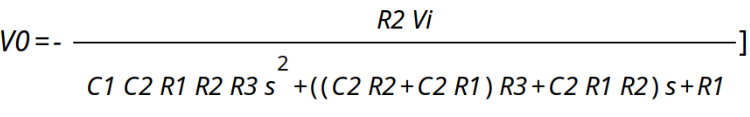
\includegraphics{v0.png}
\end{adjustbox}


\subparagraph*{Daqui criamos nossa função transferência $H$.}


\subparagraph*{}


\begin{adjustbox}{scale=0.4}
    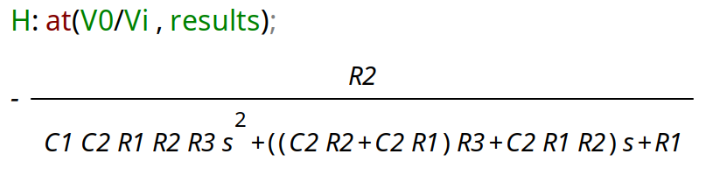
\includegraphics{H.png}
\end{adjustbox}


\subparagraph*{Agora com a função $H$ em mãos podemos substituir os valores dos resistores e do capacitor pelos que utilizaremos nos circuitos a serem analisados.}

\subsubsection{Analise do circuito 1}

\subparagraph*{Fazemos a substituicao em $H$ dos valores que utilizaremos no circuito 1.}


\begin{equation*}
    \begin{aligned}
         & C_1  = 100nF          \\
         & C_2  = 10nF           \\
         & R_1  = 47k \varOmega  \\
         & R_2  = 470k \varOmega \\
         & R_3  = 470k \varOmega
    \end{aligned}
\end{equation*}


\subparagraph*{}


\begin{adjustbox}{scale=0.34}
    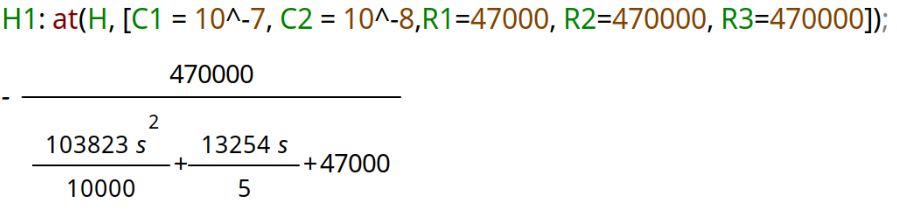
\includegraphics{H1.png}
\end{adjustbox}


\subparagraph*{Analisamos os polos e zeros da função transferência e vemos que nao ha zeros. E os polos estao abaixo:}

\subparagraph*{}

\begin{adjustbox}{scale=0.5}
    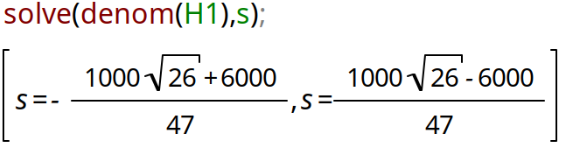
\includegraphics{H1denom.png}
\end{adjustbox}




\subparagraph*{Agora faremos graficos de Bode para analisar o comportamento da magnitude da funcao transferencia e o angulo de fase entre as saidas e entradas do circuito.}

\subparagraph*{}

\begin{figure}[h]
    \centering
    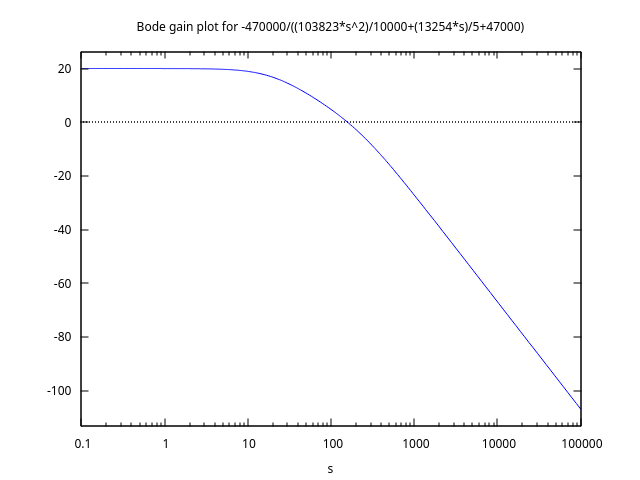
\includegraphics[width=1\columnwidth]{images/H1bodegain.png}
    \caption{Magnitude de H(s) do circuito 1.}
\end{figure}

\begin{figure}[h]
    \centering
    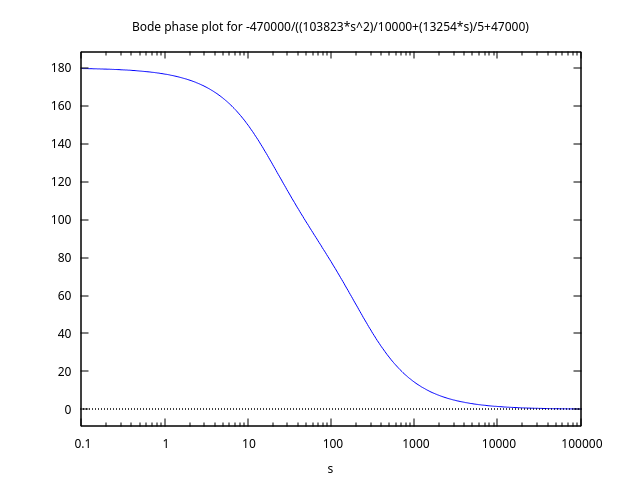
\includegraphics[width=1\columnwidth]{images/H1bodephase.png}
    \caption{Fase de H(s) do circuito 1.}
\end{figure}

\subparagraph*{}

\subparagraph*{Daqui retornei para o dominio do tempo para ter a funcao que descreve completamente o comportamento  da resposta do circuito.}
\pagebreak
\subparagraph*{}


\begin{adjustbox}{scale=0.35}
    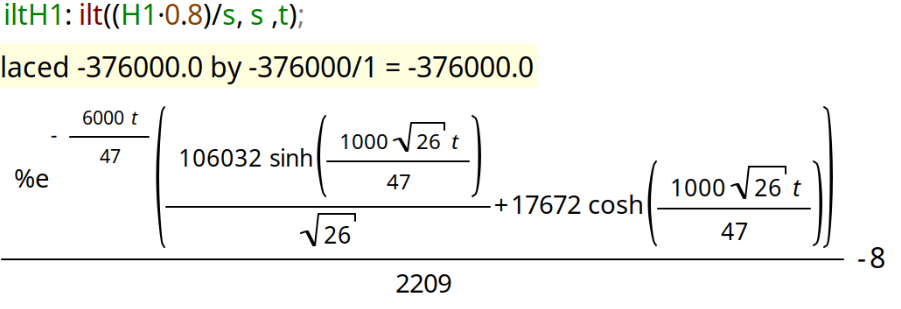
\includegraphics{iltH1.png}
\end{adjustbox}

\subparagraph*{Podemos ver que ja que todos termos exceto o $-8$ dependem de uma exponencial negativa em $t$, entao se nosso tempo tende a infinito, a resposta do circuito tende a $-8$.}

\subparagraph*{Fazendo esta analise numericamente abaixo verificamos este resultado.}

\subparagraph*{}

\begin{adjustbox}{scale=0.35}
    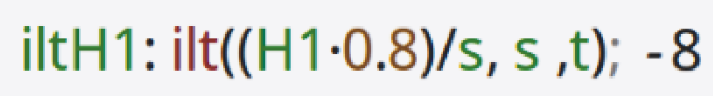
\includegraphics{limH1.png}
\end{adjustbox}

\subparagraph*{Com a funcao que descreve o comportamento do circuito no tempo em mãos podemos montar seu grafico e analisar seu comportamento para qualquer tempo.}
\subparagraph*{}

\begin{figure}[h]
    \centering
    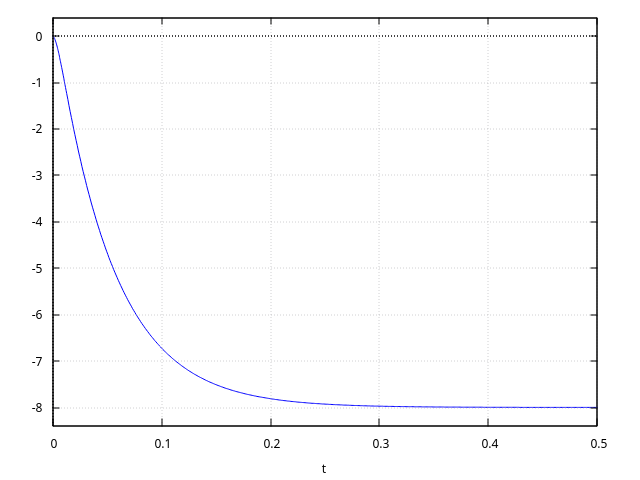
\includegraphics[width=1\columnwidth]{images/graficoH1t.png}
    \caption{Grafico de $V_0$(t) do circuito 1.}
\end{figure}


\subparagraph*{Observamos que a funcao atinge valor final de $-8V$.}

\subparagraph*{E chega a $10\%$ deste valor em $9.2ms$ e $90\%$ em $122.2ms$.}

\subsubsection{Analise do circuito 2}

\subparagraph*{Fazemos a substituicao em $H$ dos valores que utilizaremos no circuito 1.}


\begin{equation*}
    \begin{aligned}
         & C_1  = 100nF          \\
         & C_2  = 10nF           \\
         & R_1  = 470k \varOmega \\
         & R_2  = 470k \varOmega \\
         & R_3  = 47k \varOmega
    \end{aligned}
\end{equation*}


\subparagraph*{}


\begin{adjustbox}{scale=0.34}
    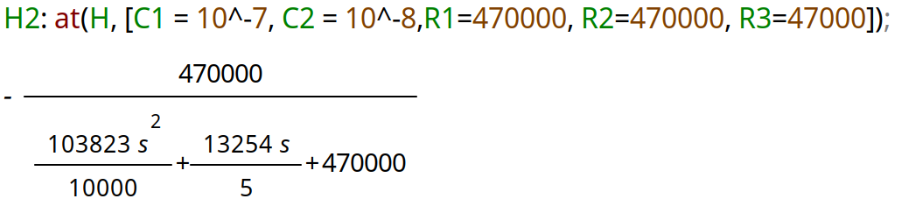
\includegraphics{H2.png}
\end{adjustbox}


\subparagraph*{Analisamos os polos e zeros da função transferência e vemos que nao ha zeros. E os polos estao abaixo:}

\subparagraph*{}

\begin{adjustbox}{scale=0.5}
    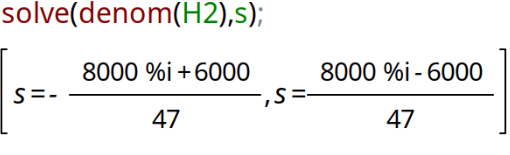
\includegraphics{H2denom.png}
\end{adjustbox}




\subparagraph*{Agora faremos graficos de Bode para analisar o comportamento da magnitude da funcao transferencia e o angulo de fase entre as saidas e entradas do circuito.}

\subparagraph*{}

\begin{figure}[h]
    \centering
    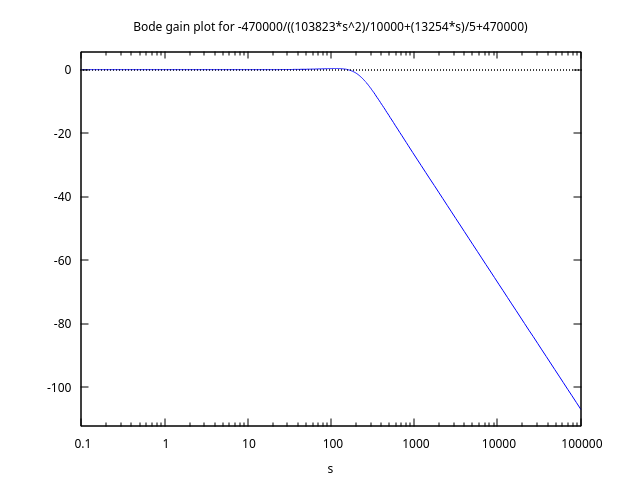
\includegraphics[width=1\columnwidth]{images/H2bodegain.png}
    \caption{Magnitude de H(s) do circuito 2.}
\end{figure}

\begin{figure}[h]
    \centering
    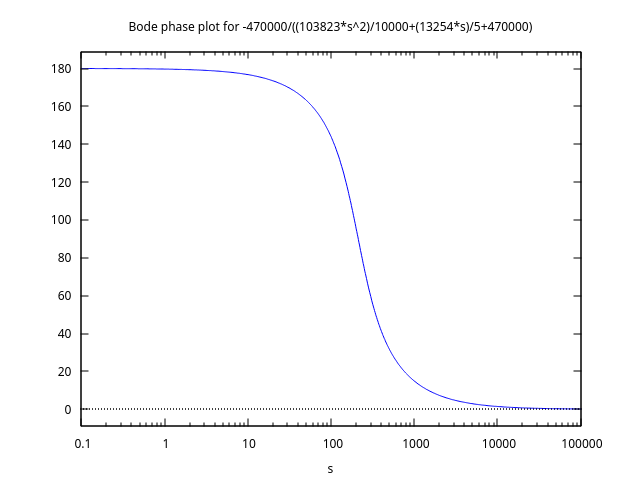
\includegraphics[width=1\columnwidth]{images/H2bodephase.png}
    \caption{Fase de H(s) do circuito 2.}
\end{figure}

\pagebreak

\subparagraph*{Daqui retornei para o dominio do tempo para ter a funcao que descreve completamente o comportamento  da resposta do circuito.}

\subparagraph*{}


\begin{adjustbox}{scale=0.35}
    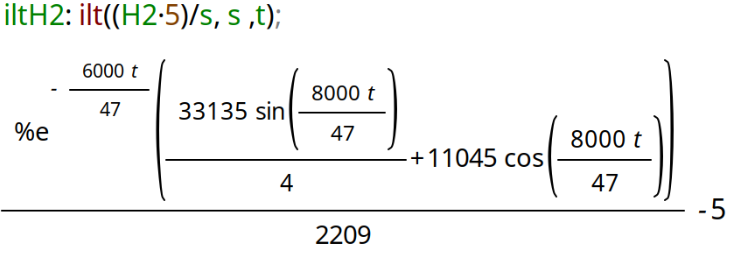
\includegraphics{iltH2.png}
\end{adjustbox}


\subparagraph*{Podemos ver que ja que todos termos exceto o $-5$ dependem de uma exponencial negativa em $t$, entao se nosso tempo tende a infinito, a resposta do circuito tende a $-5$.}

\subparagraph*{Fazendo esta analise numericamente abaixo verificamos este resultado.}

\subparagraph*{}

\begin{adjustbox}{scale=0.4}
    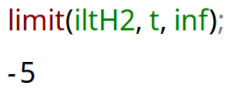
\includegraphics{limH2.png}
\end{adjustbox}

\subparagraph*{Com a funcao que descreve o comportamento do circuito no tempo em mãos podemos montar seu grafico e analisar seu comportamento para qualquer tempo.}

\newpage

\begin{figure}[h]
    \centering
    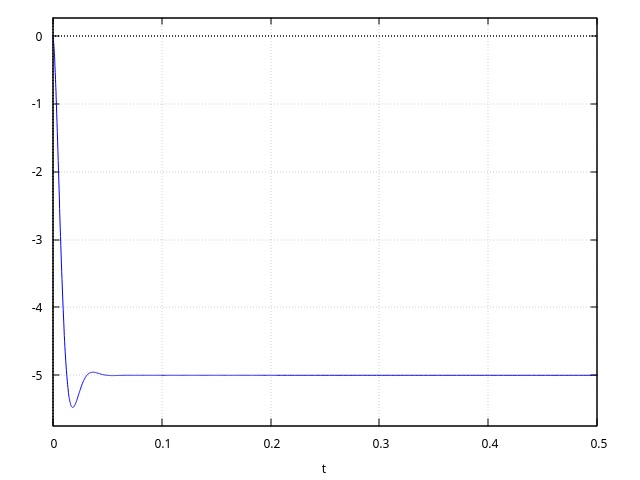
\includegraphics[width=1\columnwidth]{images/graficoH2t.png}
    \caption{Grafico de $V_0$(t) do circuito 2.}
\end{figure}

\subparagraph*{Observamos que a funcao atinge valor final de $-5V$.}

\subparagraph*{E chega a $10\%$ deste valor em $2.4ms$ e $90\%$ em $10.9ms$.}

\subparagraph*{A partir de $10.9ms$ a funcao estara contida entre $90\%$ e $110\%$ do valor final.}



\newpage




\subsection{LTSpice}

\subsubsection*{Montagem do circuito}

\paragraph*{No LTSpice montaremos o circuito e mediremos seu angulo de fase e a magnitude a funcao transferenecia, com estes valores criaremos um grafico e compararemos com o grafico de Bode.}
\subparagraph*{}
\begin{adjustbox}{scale=0.09}
    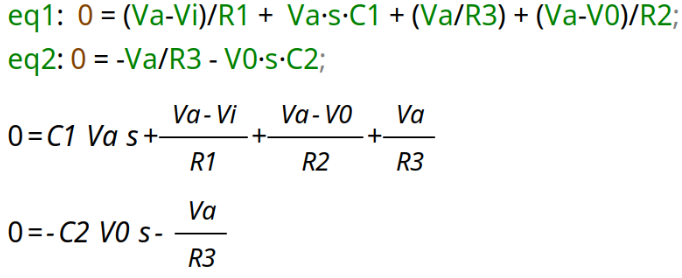
\includegraphics{eqs.png}
\end{adjustbox}


\subsubsection{Analise em $40Hz$}


\begin{adjustbox}{scale=0.09}
    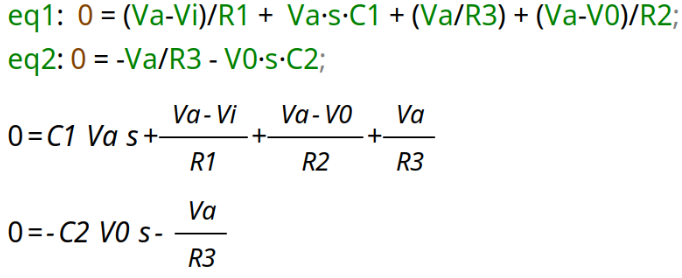
\includegraphics{eqs.png}
\end{adjustbox}


\begin{equation*}
    \begin{aligned}
         & V_f =          & 117.10115mV \\
         & V_i =          & 199.76772mV \\
         & Magnitude(H) = & 0.586186547 \\
         & Fase =         & -1.68605608
    \end{aligned}
\end{equation*}


\subsubsection{Analise em $100Hz$}


\begin{adjustbox}{scale=0.09}
    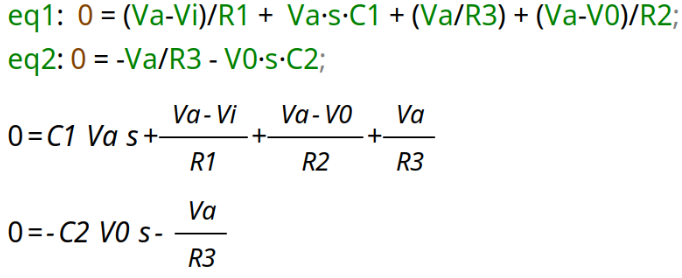
\includegraphics{eqs.png}
\end{adjustbox}


\begin{equation*}
    \begin{aligned}
         & V_f =          & 303.64554mV \\
         & V_i =          & 199.34196mV \\
         & Magnitude(H) = & 1.52323946  \\
         & Fase =         & -1.60226153
    \end{aligned}
\end{equation*}




\subsubsection{Analise em $200Hz$}


\begin{adjustbox}{scale=0.09}
    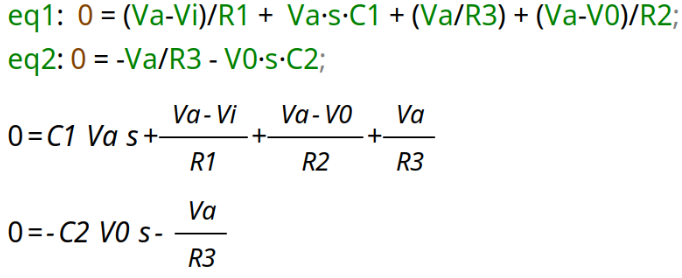
\includegraphics{eqs.png}
\end{adjustbox}


\begin{equation*}
    \begin{aligned}
         & V_f =          & 704.6312mV  \\
         & V_i =          & 199.46039mV \\
         & Magnitude(H) = & 3.53268737  \\
         & Fase =         & -1.67119113
    \end{aligned}
\end{equation*}


\subsubsection{Analise em $400Hz$}


\begin{adjustbox}{scale=0.09}
    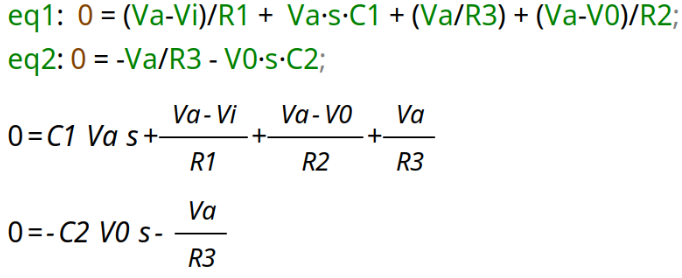
\includegraphics{eqs.png}
\end{adjustbox}


\begin{equation*}
    \begin{aligned}
         & V_f =          & 3.7148299V  \\
         & V_i =          & 199.72118mV \\
         & Magnitude(H) = & 18.6104333  \\
         & Fase =         & -2.06820459
    \end{aligned}
\end{equation*}


\subsubsection{Analise em $480Hz$}


\begin{adjustbox}{scale=0.09}
    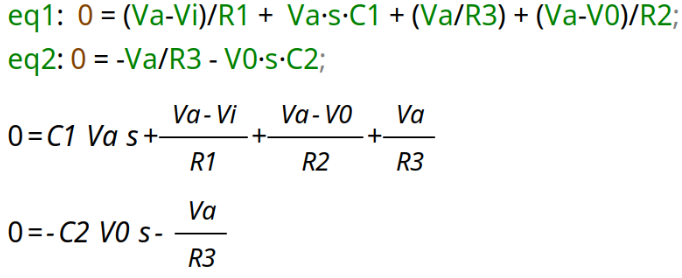
\includegraphics{eqs.png}
\end{adjustbox}


\begin{equation*}
    \begin{aligned}
         & V_f =          & 9.7253442V  \\
         & V_i =          & 199.42436mV \\
         & Magnitude(H) = & 48.7670824  \\
         & Fase =         & -3.13491022
    \end{aligned}
\end{equation*}


\subsubsection{Analise em $550Hz$}


\begin{adjustbox}{scale=0.09}
    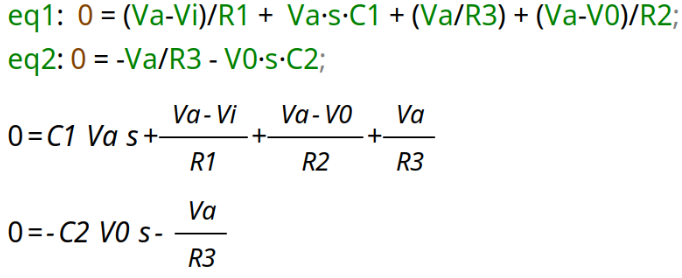
\includegraphics{eqs.png}
\end{adjustbox}


\begin{equation*}
    \begin{aligned}
         & V_f =          & 4.1496957V  \\
         & V_i =          & 199.35122mV \\
         & Magnitude(H) = & 20.8160035  \\
         & Fase =         & -2.01155708
    \end{aligned}
\end{equation*}


\subsubsection{Analise em $1100Hz$}


\begin{adjustbox}{scale=0.09}
    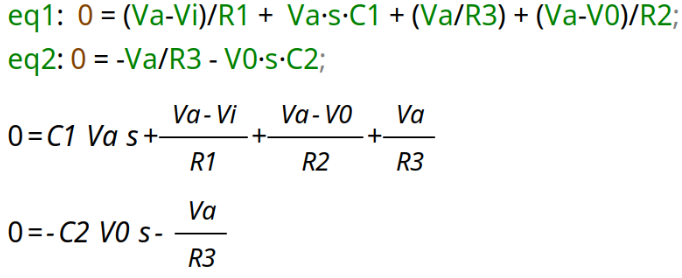
\includegraphics{eqs.png}
\end{adjustbox}


\begin{equation*}
    \begin{aligned}
         & V_f =          & 724.81506mV \\
         & V_i =          & 199.55853mV \\
         & Magnitude(H) = & 3.6320926   \\
         & Fase =         & -1.65494612
    \end{aligned}
\end{equation*}



\subsubsection{Tabela de resultados}






\subparagraph*{}


\begin{center}
    \begin{tabular}{ |c|c|c| }
        \hline
        Freq (Hz) & | H (jw) |  & Fase (H)      \\
        40        & 0.586186547 & $-1.68605608$ \\
        100       & 1.52323946  & $-1.60226153$ \\
        200       & 3.53268737  & $-1.67119113$ \\
        400       & 18.6104333  & $-2.06820459$ \\
        480       & 48.7670824  & $-3.1349102$  \\
        550       & 20.8160035  & $-2.01155708$ \\
        1100      & 3.6320926   & $-1.65494612$ \\
        2200      & 1.55687244  & $-4.68032157$ \\
        5500      & 0.595261852 & $1.60939706$  \\
        11000     & 0.296616925 & $-4.65829159$ \\
        \hline
    \end{tabular}
\end{center}
\newpage
\section{Medicoes em laboratorio}


\paragraph{Vamos inicialmente fazer as medições dos componentes a serem usados.}


\subsection{Tabela de componentes}


\begin{equation*}
    \begin{aligned}
        C_1 & = 104.89nF    \\
        C_2 & = 101.28nF    \\
        R_1 & = 465.1 omega \\
        R_2 & = 473.7 omega \\
        R_3 & = 46.25 omega \\
    \end{aligned}
\end{equation*}


\subsection{Médicos no osciloscopio}


\subsubsection*{Analise em $40Hz$}
\subparagraph*{}


\begin{adjustbox}{scale=0.18}
    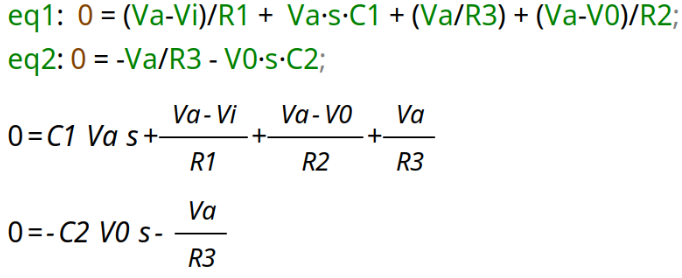
\includegraphics{eqs.png}
\end{adjustbox}


\begin{equation*}
    \begin{aligned}
         & V_f =          & 0.565V     \\
         & V_i =          & 0.092V     \\
         & Magnitude(H) = & 0.473      \\
         & Fase =         & -1.5833627
    \end{aligned}
\end{equation*}




\subsubsection{Analise em $100Hz$}
\subparagraph*{}


\begin{adjustbox}{scale=0.18}
    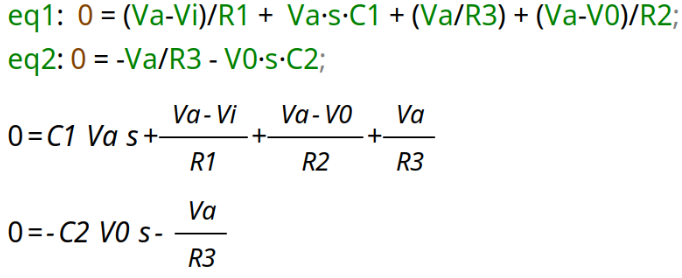
\includegraphics{eqs.png}
\end{adjustbox}


\begin{equation*}
    \begin{aligned}
         & V_f =          & 1.52V       \\
         & V_i =          & 0.09425V    \\
         & Magnitude(H) = & 1.42575     \\
         & Fase =         & -1.57079633
    \end{aligned}
\end{equation*}


\subsubsection{Analise em $200Hz$}
\subparagraph*{}


\begin{adjustbox}{scale=0.18}
    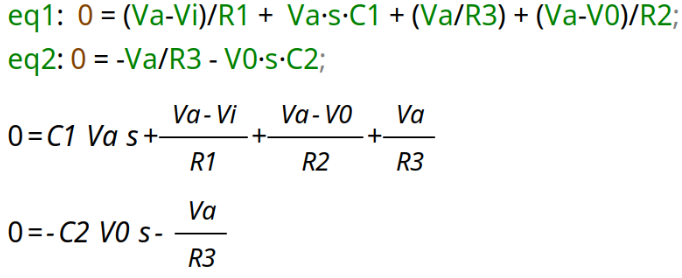
\includegraphics{eqs.png}
\end{adjustbox}


\begin{equation*}
    \begin{aligned}
         & V_f =          & 3.5425V     \\
         & V_i =          & 0.097V      \\
         & Magnitude(H) = & 3.4455      \\
         & Fase =         & -1.55822996
    \end{aligned}
\end{equation*}


\subsubsection{Analise em $400Hz$}
\subparagraph*{}


\begin{adjustbox}{scale=0.18}
    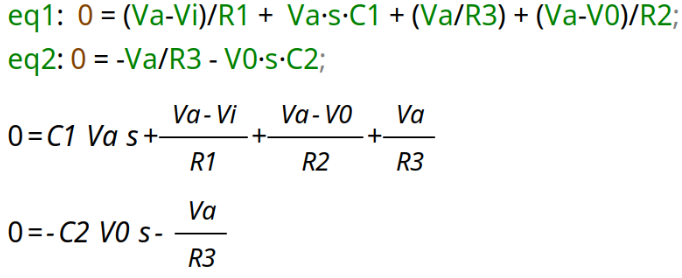
\includegraphics{eqs.png}
\end{adjustbox}


\begin{equation*}
    \begin{aligned}
         & V_f =          & 21.5V       \\
         & V_i =          & 0.106V      \\
         & Magnitude(H) = & 21.394      \\
         & Fase =         & -1.98548656
    \end{aligned}
\end{equation*}


\begin{equation*}
    \begin{aligned}
         & V_f =          & 0.09V       \\
         & V_i =          & 199.57788mV \\
         & Magnitude(H) = & 0.04325V    \\
         & Fase =         & 1.24407069
    \end{aligned}
\end{equation*}


\subsubsection{Tabela de resultados}


\subparagraph*{}


\begin{center}
    \begin{tabular}{ |c|c|c| }
        \hline
        Freq (Hz) & | H (jw) | & Fase (H)      \\
        40        & 0.473      & $-1.5833627$  \\
        100       & 1.42575    & $-1.57079633$ \\
        200       & 3.4455     & $-1.55822996$ \\
        400       & 21.394     & $-1.98548656$ \\
        480       & 36.65      & $-3.40799971$ \\
        550       & 16.71800   & $2.07345115$  \\
        1100      & 3.6320926  & $ 1.58964588$ \\
        2200      & 0.575      & $1.65876092$  \\
        5500      & 0.61       & $0.552920307$ \\
        11000     & 0.04325    & $1.24407069$  \\
        \hline
    \end{tabular}
\end{center}


\subsection{Comparação com valores teóricos}


\subparagraph*{Podemos ver que os valores de magnitude ficaram coerentes com ambas análises teóricas, e os de fases para frequências baixas também, mas tive problemas para entender o sentido do sinal da fase a medida que a frequência subia.}


\subsection{Gráficos}


\subsubsection{Escala log-log da magnitude de H(jw) e f}


\begin{adjustbox}{scale=0.70}
    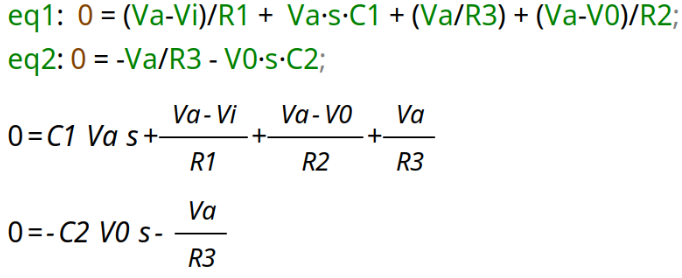
\includegraphics{eqs.png}
\end{adjustbox}


\subsubsection{Escala semilog da fase de H(jw) e f}
\begin{adjustbox}{scale=0.70}
    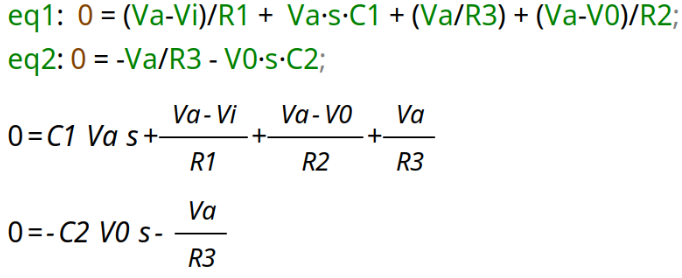
\includegraphics{eqs.png}
\end{adjustbox}


\section{Conclusões}


\subparagraph*{Conseguimos com sucesso fazer a análise numérica por dois meios, utilizando o LTSpice e WxMaxima, e comparamos os resultados.}


\subparagraph*{Nos resultados práticos, a magnitude da função transferência foi coerente com os resultados esperados, porém a fase em frequências baixas se manteve coerente, porém em frequências altas ela se tornou inconsistente.}


\subparagraph*{Creio que por erros das minhas medidas, eu não fui consistente em usar o mesmo cursor na mesma onda de entrada ou saída.}


\subparagraph*{A frequência de saída começou adiantada em relação a frequência de entrada, e à medida que aumentamos a frequência ela se atrasa até que é ultrapassada pela entrada.}


\subparagraph*{Creio que isso faria com que a fase se inverta.}


\subparagraph*{Mas em suma creio que tivemos sucesso em nos familiarizar com as ferramentas de análise de circuitos elétricos numéricos.}


\end{document}